\documentclass[border=3pt]{standalone}
% Preâmbulo compartilhado pelos diagramas TikZ da aula 7 (Filtros Não Paramétricos)
\usepackage[T1]{fontenc}
\usepackage[utf8]{inputenc}
\usepackage{lmodern}
\usepackage{amsmath}
\usepackage{xcolor}
\usepackage{tikz}
\usetikzlibrary{arrows.meta,angles,quotes,decorations.pathmorphing,calc,
                positioning,shapes.geometric,shapes.misc,backgrounds,fit,
                math}

% Paleta (mesma dos SVGs originais)
\definecolor{dblue}{HTML}{2A5B8C}
\definecolor{dorange}{HTML}{B3541E}
\definecolor{dgreen}{HTML}{4A7C59}
\definecolor{dred}{HTML}{9C4B4B}
\definecolor{dcream}{HTML}{F4F1EA}
\definecolor{dshade}{HTML}{DDD7C9}

% Função gaussiana (não normalizada por padrão de escala visual)
\pgfmathdeclarefunction{gauss}{3}{%
  \pgfmathparse{1/(#3*sqrt(2*pi))*exp(-((#1-#2)^2)/(2*#3^2))}%
}

% Estilos comuns (prefixo d... para não colidir com chaves internas do pgf)
\tikzset{
  >={Stealth[length=2mm]},
  dguide/.style={gray!55, dashed, line width=0.4pt},
  daxis/.style={gray!60, line width=0.7pt, ->},
  dbody/.style={fill=black!3, draw=black!80, line width=1pt},
  dacc/.style={draw=dblue, line width=1pt},
  dlbl/.style={black!55, font=\small},
  dsub/.style={black!45, font=\footnotesize},
  dstate/.style={circle, draw=black!80, fill=dcream, line width=1pt,
                 minimum size=17mm, font=\large, inner sep=1pt},
  dobs/.style={circle, draw=black!80, fill=dshade, line width=1pt,
               minimum size=14mm, font=\large, inner sep=1pt},
  dbox/.style={rounded corners=2pt, draw=black!80, fill=dcream, line width=1pt,
               align=center, inner sep=6pt},
  dop/.style={circle, draw=black!80, fill=white, line width=1pt,
              minimum size=6mm, inner sep=0pt, font=\small},
  dtrans/.style={->, dblue, line width=1pt},
  dmeas/.style={->, dorange, line width=1pt},
  dcurve/.style={line width=1pt, dblue},
  dcurveb/.style={line width=1.4pt, dorange},
}

\begin{document}
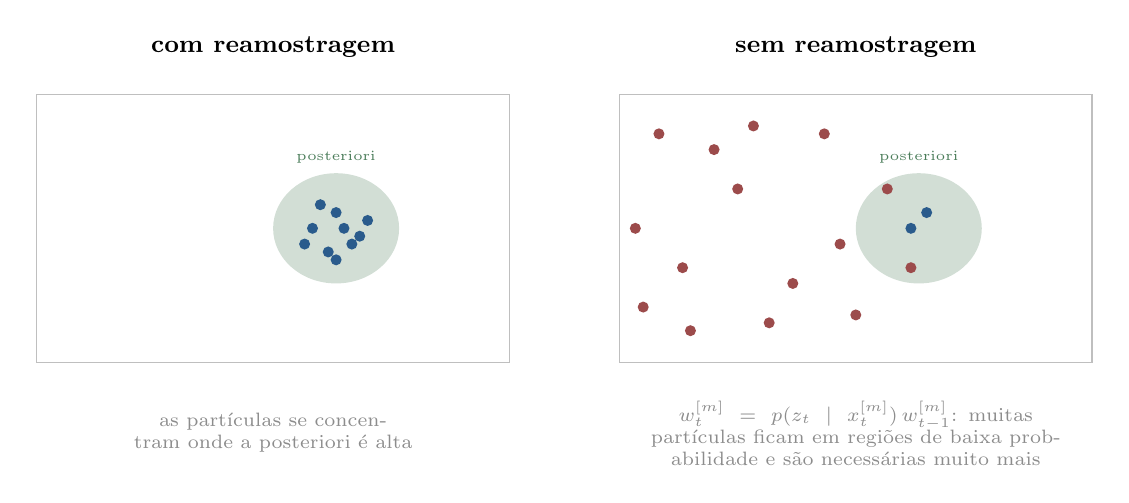
\begin{tikzpicture}[x=1cm,y=1cm]
  \newcommand{\painel}[2]{\begin{scope}[shift={(#1)}] \draw[black!25] (0,0) rectangle (6,3.4); \node[font=\small\bfseries] at (3,4.0) {#2};
    \fill[dgreen!25] (3.8,1.7) ellipse (0.8 and 0.7); \node[dgreen, font=\tiny] at (3.8,2.6) {posteriori};\end{scope}}
  \painel{0,0}{com reamostragem}
  \foreach \x/\y in {3.5/1.7,3.8/1.9,4.0/1.5,3.7/1.4,4.2/1.8,3.6/2.0,3.9/1.7,4.1/1.6,3.4/1.5,3.8/1.3} { \fill[dblue] (\x,\y) circle (0.07); }
  \painel{7.4,0}{sem reamostragem}
  \foreach \x/\y in {7.7/0.7,8.6/2.7,9.3/0.5,10.0/2.9,8.2/1.2,9.6/1.0,10.4/0.6,8.9/2.2,7.9/2.9,10.8/2.2,9.1/3.0,11.1/1.2,10.2/1.5,7.6/1.7,8.3/0.4} { \fill[dred] (\x,\y) circle (0.07); }
  \foreach \x/\y in {11.1/1.7,11.3/1.9} { \fill[dblue] (\x,\y) circle (0.07); }
  \node[dsub, font=\scriptsize, align=center, text width=6cm] at (3,-0.9) {as partículas se concentram onde a posteriori é alta};
  \node[dsub, font=\scriptsize, align=center, text width=6cm] at (10.4,-0.9) {$w_t^{[m]}=p(z_t\mid x_t^{[m]})\,w_{t-1}^{[m]}$: muitas partículas ficam em regiões de baixa probabilidade e são necessárias muito mais};
\end{tikzpicture}
\end{document}
